\documentclass[10pt,twocolumn]{article}

% ── Layout ──────────────────────────────────────────────────────────
\usepackage[margin=0.65in,top=0.65in,bottom=0.65in]{geometry}

% ── Typography ──────────────────────────────────────────────────────
\usepackage[T1]{fontenc}
\usepackage{mathpazo}              % Palatino text + math
\usepackage[scaled=0.88]{helvet}   % Helvetica for sans-serif
\usepackage{courier}               % Courier for mono
\usepackage{microtype}             % Optical adjustments
\linespread{1.05}                  % Palatino reads better with slight spread

% ── Packages ────────────────────────────────────────────────────────
\usepackage{graphicx}
\usepackage{booktabs}
\usepackage{enumitem}
\usepackage{caption}
\usepackage{float}
\usepackage[table]{xcolor}
\usepackage{titlesec}
\usepackage{fancyhdr}
\usepackage{tcolorbox}
\usepackage{tikz}
\usetikzlibrary{arrows.meta,positioning,shapes.geometric,fit,backgrounds,calc}
\usepackage[colorlinks,linkcolor=NavyBlue,citecolor=NavyBlue,urlcolor=NavyBlue]{hyperref}

% ── Colors ──────────────────────────────────────────────────────────
\definecolor{NavyBlue}{RGB}{0,51,102}
\definecolor{LightGray}{RGB}{245,245,245}
\definecolor{MedGray}{RGB}{128,128,128}
\definecolor{TableShade}{RGB}{248,248,252}

% ── Section formatting ──────────────────────────────────────────────
\setlength{\parskip}{4pt plus 1pt}
\setlength{\parindent}{0pt}
\setlist{nosep,leftmargin=*}

\titlespacing*{\section}{0pt}{10pt}{4pt}
\titlespacing*{\subsection}{0pt}{8pt}{2pt}
\titleformat{\section}{\normalfont\bfseries\normalsize\scshape}{\thesection}{0.6em}{}
\titleformat{\subsection}{\normalfont\bfseries\small}{\thesubsection}{0.5em}{}

% ── Captions ────────────────────────────────────────────────────────
\setlength{\abovecaptionskip}{6pt}
\setlength{\belowcaptionskip}{2pt}
\captionsetup{font=small,labelfont={bf,small},labelsep=period,format=hang}

% ── Table row spacing ──────────────────────────────────────────────
\renewcommand{\arraystretch}{1.15}

% ── Headers/footers ────────────────────────────────────────────────
\pagestyle{fancy}
\fancyhf{}
\renewcommand{\headrulewidth}{0pt}
\fancyfoot[C]{\small\thepage}

% ── Prompt boxes ───────────────────────────────────────────────────
\tcbset{
  promptbox/.style={
    colback=LightGray,
    colframe=LightGray,
    boxrule=0pt,
    arc=2pt,
    left=8pt,right=8pt,top=6pt,bottom=6pt,
    fontupper=\small\ttfamily,
  }
}

% ═══════════════════════════════════════════════════════════════════
\begin{document}

% ── Title block ────────────────────────────────────────────────────
\twocolumn[{
\begin{center}
\vspace{4pt}
{\LARGE\bfseries Autoreason: Autoresearch for Subjective Domains}\\[10pt]
{\normalsize shl0ms}\\[2pt]
{\small\textcolor{MedGray}{\url{https://github.com/NousResearch/autoreason}}}\\[12pt]
\end{center}
}]

% ── Abstract ───────────────────────────────────────────────────────
\noindent\textbf{\scshape Abstract.}\enspace
We introduce autoreason, a method for iterative LLM refinement in subjective domains where no objective metric exists. Each iteration produces three competing versions of a document (the incumbent, an adversarial revision, and a synthesis), evaluated by a blind judge panel. Fresh isolated agents, Borda count aggregation, and conservative tiebreaking construct a subjective fitness function through the evaluation process itself. With claude-sonnet-4 across 5~task types, autoreason ranked first or second in every 7-judge blind comparison, winning 3/5~outright. Chain-of-thought judging accelerates convergence 3$\times$ on Task~1 (1.5$\times$ on Task~2); Monte Carlo analysis suggests 80\% convergence with consistent quality (though $n{=}5$ limits precision); game-theoretic analysis suggests near-transitive preferences.

With a stronger model (Sonnet~4.6), the method fails on open-ended tasks: synthesis consistently outcompetes the incumbent, preventing convergence. Eight remedy experiments identify the root cause as \textit{scope}, not evaluation methodology. On a scope-constrained task (500-word pitch), the same stronger model converges in 10~passes and wins a blind comparison against all baselines. This result comes from a single constrained task and requires further validation across other task types and constraint forms before any general conclusion can be drawn. Autoreason's effectiveness depends on the interaction between evaluation methodology and task specification: the synthesis operator needs a bounded improvement space to reach a quality ceiling.

\vspace{6pt}
\hrule
\vspace{6pt}

\section{Introduction}

LLMs exhibit systematic failures when iterating on subjective work: sycophancy, overcriticism, overcompromise, authorship bias, scope drift, and context collapse. Even in code generation, iterative refinement leads to progressive degradation~\cite{slopcodebench}. Self-Refine~\cite{selfrefine} demonstrates that single-agent critique-and-revise loops can improve outputs but provides no mechanism to detect when revisions make things worse. Huang et al.~\cite{huang2023} show LLMs cannot reliably self-correct without external feedback, motivating our external judge panel.

We present autoreason, extending Karpathy's autoresearch~\cite{autoresearch} to subjective domains. Each iteration produces three competing versions: the incumbent~(A), an adversarial revision~(B), and a synthesis~(AB), evaluated by a blind judge panel. The method constructs a fitness function through the evaluation process itself.

We tested two modes. \textbf{Single pass}: one cycle through critic $\to$ B $\to$ AB $\to$ judge (5~LLM calls). \textbf{Convergence loop}: repeats the cycle with a full judge panel until the incumbent survives consecutive challenges. As we show in Section~\ref{sec:v1}, the single pass does not outperform simpler baselines; autoreason's value emerges from iteration. We further show that with stronger models, the method's effectiveness depends on task scope: scope constraints restore convergence and quality where unconstrained tasks fail (Section~\ref{sec:scaling}).

\section{Method}

\begin{figure*}[t]
\centering
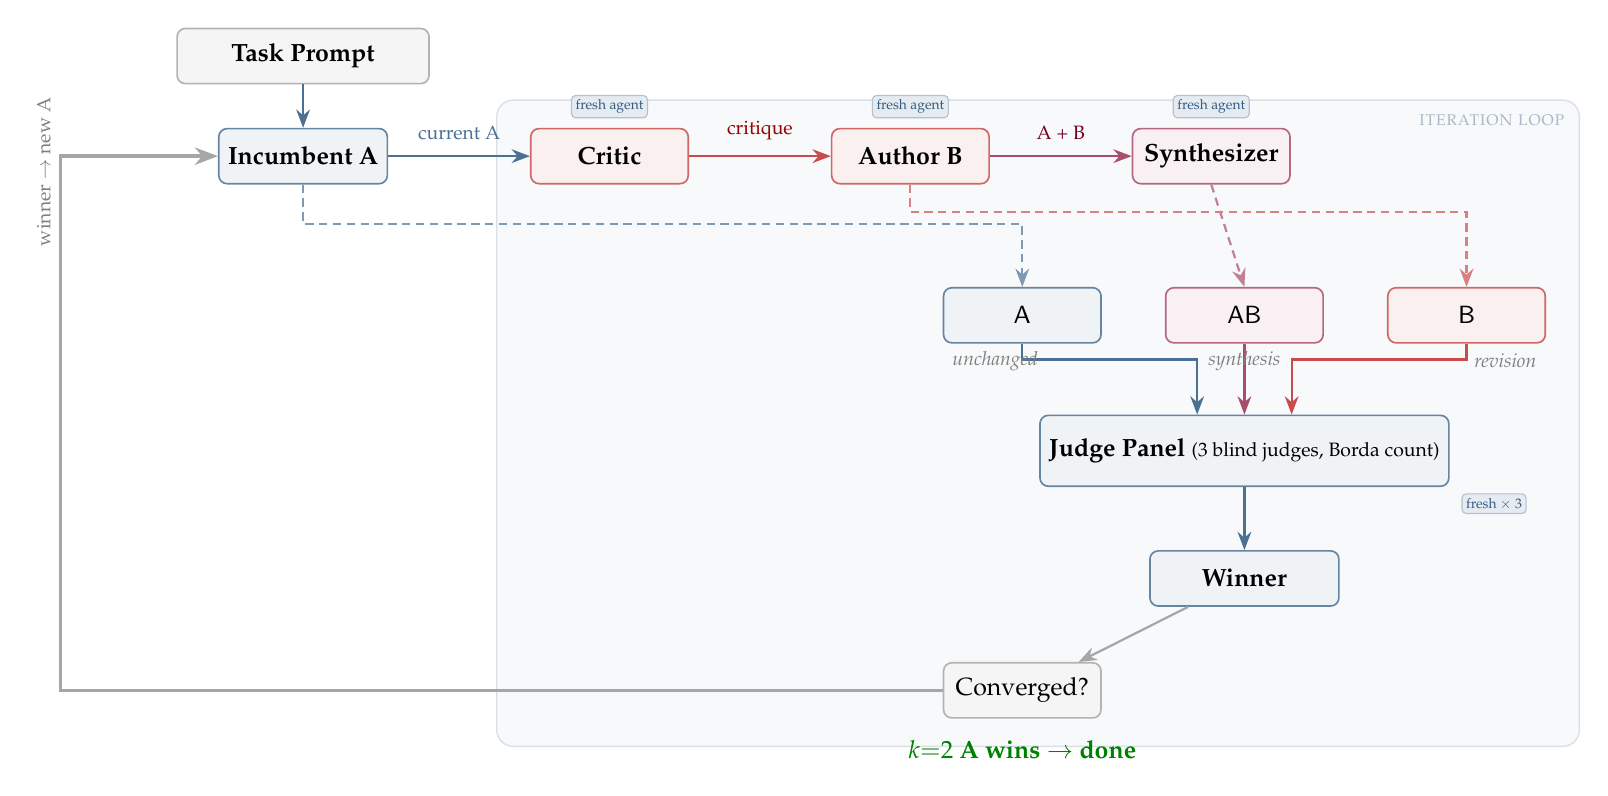
\begin{tikzpicture}[
    >=Stealth,
    node distance=0.6cm and 1.2cm,
    box/.style={rectangle, rounded corners=3pt, draw=#1!60, fill=#1!6,
                minimum height=0.7cm, minimum width=2.0cm,
                font=\small, text=black, line width=0.6pt},
    box/.default=NavyBlue,
    arr/.style={->, thick, color=#1!70},
    arr/.default=NavyBlue,
    dasharr/.style={->, densely dashed, thick, color=#1!50},
    dasharr/.default=NavyBlue,
]

% ── Task prompt anchor ──
\node[box=MedGray, minimum width=3.2cm, fill=LightGray, draw=MedGray!60]
    (task) {\textbf{Task Prompt}};

% ── Incumbent A ──
\node[box, below=0.55cm of task] (A) {\textbf{Incumbent A}};

% ── Critic ──
\node[box=red!70!black, right=1.8cm of A] (critic) {\textbf{Critic}};

% ── Author B ──
\node[box=red!70!black, right=1.8cm of critic] (authorB) {\textbf{Author B}};

% ── Synthesizer ──
\node[box=purple!70!black, right=1.8cm of authorB] (synth) {\textbf{Synthesizer}};

% ── Three candidates: A, AB, B order ──
\node[box, below=1.3cm of synth, xshift=-2.4cm] (candA) {\textsf{A}};
\node[box=purple!70!black, right=0.8cm of candA] (candAB) {\textsf{AB}};
\node[box=red!70!black, right=0.8cm of candAB] (candB) {\textsf{B}};

% ── Judge panel ──
\node[box=NavyBlue, below=0.9cm of candAB, minimum width=4.8cm, minimum height=0.9cm]
    (judge) {\textbf{Judge Panel} {\scriptsize (3 blind judges, Borda count)}};

% ── Winner decision ──
\node[box=NavyBlue, below=0.8cm of judge, minimum width=2.4cm] (winner) {\textbf{Winner}};

% ── Convergence check ──
\node[box=MedGray, fill=LightGray, draw=MedGray!60, below left=0.7cm and 0.6cm of winner,
      minimum width=2.0cm] (conv) {Converged?};

% ── Arrows: main pipeline (top row) ──
\draw[arr] (task) -- (A);
\draw[arr] (A) -- (critic);
\draw[arr=red!70!black] (critic) -- (authorB);
\draw[arr=purple!70!black] (authorB) -- (synth);

% ── Edge labels on pipeline arrows ──
\node[font=\scriptsize, text=NavyBlue!70, above=0.08cm] at ($(A.east)!0.5!(critic.west)$) {current A};
\node[font=\scriptsize, text=red!60!black, above=0.08cm] at ($(critic.east)!0.5!(authorB.west)$) {critique};
\node[font=\scriptsize, text=purple!60!black, above=0.08cm] at ($(authorB.east)!0.5!(synth.west)$) {A + B};

% ── Arrows: candidates down (dashed) ──
\draw[dasharr] (A.south) -- ++(0,-0.5) -| (candA.north);
\draw[dasharr=purple!70!black] (synth.south) -- (candAB.north);
\draw[dasharr=red!70!black] (authorB.south) -- ++(0,-0.35) -| (candB.north);

% ── Arrows: candidates to judge ──
\draw[arr] (candA.south) -- ++(0,-0.2) -| ([xshift=-0.6cm]judge.north);
\draw[arr=purple!70!black] (candAB.south) -- (judge.north);
\draw[arr=red!70!black] (candB.south) -- ++(0,-0.2) -| ([xshift=0.6cm]judge.north);

% ── Judge to winner ──
\draw[arr] (judge) -- (winner);

% ── Winner to convergence check ──
\draw[arr=MedGray] (winner) -- (conv);

% ── Loop back arrow: route along far left, clear of all elements ──
\coordinate (loopleft) at ([xshift=-2.0cm]A.west);
\draw[arr=MedGray, line width=1.2pt]
    (conv.west) -| (loopleft) -- (A.west);
\node[font=\scriptsize, text=MedGray, rotate=90, anchor=south]
    at ([xshift=-2.0cm, yshift=-0.2cm]A.west) {winner $\to$ new A};

% ── Convergence exit ──
\node[font=\small\bfseries, text=green!50!black, below=0.15cm of conv] {$k{=}2$ A wins $\to$ \textrm{done}};

% ── Fresh agent badges: positioned clearly above each role ──
\begin{scope}[every node/.style={font=\tiny, rounded corners=1.5pt,
    fill=NavyBlue!10, draw=NavyBlue!30, inner sep=1.5pt, text=NavyBlue!80}]
    \node[above=0.12cm of critic] {fresh agent};
    \node[above=0.12cm of authorB] {fresh agent};
    \node[above=0.12cm of synth] {fresh agent};
    \node[below right=0.08cm and 0.15cm of judge.south east,
          anchor=north west] {fresh $\times$ 3};
\end{scope}

% ── Role descriptions: positioned below candidates, clear of arrows ──
\node[font=\scriptsize\itshape, text=MedGray, anchor=west]
    at ([yshift=-0.22cm]candA.south west) {unchanged};
\node[font=\scriptsize\itshape, text=MedGray, anchor=center]
    at ([yshift=-0.22cm]candAB.south) {synthesis};
\node[font=\scriptsize\itshape, text=MedGray, anchor=east]
    at ([yshift=-0.22cm]candB.south east) {revision};

% ── Loop region background ──
\begin{scope}[on background layer]
\node[fit=(critic)(candA)(candB)(judge)(winner)(conv),
      rounded corners=6pt, fill=NavyBlue!3, draw=NavyBlue!15,
      inner xsep=12pt, inner ysep=10pt, line width=0.5pt] (loopbg) {};
\node[font=\scriptsize\scshape, text=NavyBlue!35,
      anchor=north east] at ([xshift=-2pt, yshift=-2pt]loopbg.north east) {iteration loop};
\end{scope}

\end{tikzpicture}
\caption{The autoreason loop. Each pass evaluates three candidates: the unchanged incumbent~(A), a synthesis~(AB), and an adversarial revision~(B). A blind judge panel selects the winner via Borda count. If A survives $k{=}2$ consecutive passes, the loop terminates. Every role uses a fresh, isolated agent.}
\label{fig:method}
\end{figure*}

\textbf{Critic.}\enspace A fresh agent identifies problems in the current incumbent~A. Finds problems only; no fixes. Optionally receives ground-truth data for fact-checking (Section~\ref{sec:paper}).

\textbf{Author~B.}\enspace A fresh agent revises A based on the critique. Sees the task, A, and the critique. No drafting history.

\textbf{Synthesizer.}\enspace A fresh agent receives A and B with randomized labels. Produces AB by taking the strongest elements of each.

\textbf{Judge Panel.}\enspace 3 fresh agents rank A, AB, B via Borda count (3/2/1 points). Randomized labels and presentation order. Conservative tiebreak: incumbent wins ties. Convergence at $k{=}2$ consecutive A wins. We use 3 judges in-loop to balance per-pass cost against evaluation stability, and 7 judges for final blind comparisons to increase statistical power where cost is amortized over a single evaluation.

Every role is a fresh, isolated agent with no shared context. The original task prompt anchors all evaluation. We chose $k{=}2$ because $k{=}1$ led to premature termination on noisy judgments in early experiments, while $k{=}2$ provided a stable stopping point across all tested runs; $k{=}3$ would increase cost without meaningfully changing outcomes given the Elo plateau analysis (Section~\ref{sec:retro}). Temperature was set to 0.8 for authors (encouraging diverse revisions) and 0.3 for judges (encouraging consistent evaluation); these values were chosen based on preliminary runs and not formally ablated. Exact prompts are provided in Appendix~\ref{app:prompts}.

\subsection{Formal Framing}

Let $d_t$ denote the incumbent document at pass~$t$. Each pass produces candidates $\{d_t, B(d_t), S(d_t, B(d_t))\}$ where $B$ is the adversarial revision operator and $S$ is the synthesis operator. A judge panel $J$ defines a stochastic preference relation: $J(x, y) \in [0,1]$ is the probability that $x$ is ranked above $y$. The winner is selected by Borda aggregation over $n$ judges:

$$d_{t+1} = \arg\max_{c \in \{A, B, AB\}} \sum_{i=1}^{n} (3 - r_i(c))$$

where $r_i(c)$ is judge $i$'s rank for candidate $c$, with ties broken in favor of~$d_t$.

This defines a Markov chain over document states. Convergence ($d_{t+1} = d_t$ for $k$ consecutive passes) corresponds to an absorbing state. By the Condorcet jury theorem, if each judge independently identifies the better document with $p > 0.5$, panel accuracy increases with~$n$. However, same-model judges share systematic biases, bounding effective independence below~$n$.

The structure is loosely analogous to PSRO~\cite{psro}: each pass adds a candidate to an empirical game, but autoreason lacks PSRO's full meta-strategy computation and operates over documents rather than policies. Our retroactive analysis (Section~\ref{sec:retro}) examines this framing empirically: preferences are near-transitive across 91~passes (1.1\% Condorcet cycle rate), and Elo ratings plateau early, consistent with the Markov chain reaching its absorbing state.

\section{Experiments}

All experiments used claude-sonnet-4-20250514 (temp=0.8 authors, 0.3 judges, max\_tokens=4096) unless otherwise noted. Five tasks: (1)~go-to-market strategy, (2)~notification system design, (3)~remote work policy, (4)~competitive positioning, (5)~incident response. Each task ran autoreason to convergence ($k{=}2$) plus four baselines at 15 passes each from the same initial output, evaluated by a 7-judge blind panel. The paper-writing experiment (Section~\ref{sec:paper}) used claude-opus-4. Scaling experiments (Section~\ref{sec:scaling}) used claude-sonnet-4-6.

\textbf{Baselines.}\enspace We compared against four iterative prompting strategies, each applied for 15 passes from the same initial document: (1)~\textit{Conservative}: ``Make minimal improvements while preserving what works''; (2)~\textit{Improve this}: ``Improve this document'' with no further guidance; (3)~\textit{Harsh critic}: ``Critically evaluate and rewrite, fixing all weaknesses''; (4)~\textit{Critique \& revise}: a two-step loop where the model first produces a structured critique, then revises the document to address it (closest to Self-Refine~\cite{selfrefine}). All baselines use a single agent per pass with no judge panel or adversarial structure. Baseline prompts are provided in Appendix~\ref{app:prompts}.

\textbf{Compute budget.}\enspace Autoreason requires ${\sim}$6 LLM calls per pass (critic, author~B, synthesizer, 3 judges) and typically runs 10--25 passes to convergence (${\sim}$60--150 calls per task), while each baseline requires ${\sim}$1 call per pass (${\sim}$15 calls total). This roughly 6$\times$ per-pass cost (and larger total cost due to more passes) is a real tradeoff; autoreason trades compute for evaluation quality.

\section{Results}

\subsection{Single Pass vs.\ Iteration}
\label{sec:v1}

\begin{table}[H]
\centering
\small
\begin{tabular}{@{}lcccccc@{}}
\toprule
\textbf{Method} & \textbf{Calls} & \textbf{T1} & \textbf{T2} & \textbf{T3} & \textbf{T4} & \textbf{T5} \\
\midrule
\rowcolor{TableShade}
Harsh critic & 1 & \textbf{30} & \textbf{31} & 23 & \textbf{30} & \textbf{31} \\
Critique \& rev. & 1 & \textbf{30} & 30 & \textbf{31} & 28 & 23 \\
\rowcolor{TableShade}
Autoreason & 5 & 24 & 22 & 24 & 17 & 24 \\
Improve this & 1 & 14 & 14 & 18 & 23 & 20 \\
\rowcolor{TableShade}
Conservative & 1 & 7 & 8 & 9 & 7 & 7 \\
\bottomrule
\end{tabular}
\caption{Single-pass Borda scores (max~35). Bold indicates task winner. Autoreason places 3rd at 5$\times$ the cost.}
\label{tab:v1}
\end{table}

\begin{table}[H]
\centering
\small
\begin{tabular}{@{}lccccc@{}}
\toprule
\textbf{Method} & \textbf{T1} & \textbf{T2} & \textbf{T3} & \textbf{T4} & \textbf{T5} \\
\midrule
\rowcolor{TableShade}
\textbf{Autoreason} & \textbf{35} & 19 & \textbf{29} & 25 & \textbf{31} \\
Critique \& rev. & 13 & \textbf{22} & 26 & \textbf{32} & 19 \\
\rowcolor{TableShade}
Harsh critic & 18 & 19 & 27 & 20 & 26 \\
Conservative & 21 & 19 & 15 & 18 & 15 \\
\rowcolor{TableShade}
Improve this & 18 & 11 & 8 & 10 & 14 \\
\bottomrule
\end{tabular}
\caption{Iterative Borda scores (max~35) at 15~passes. Autoreason wins tasks 1, 3,~5; critique-and-revise wins tasks 2,~4.}
\label{tab:multi}
\end{table}

Single-pass autoreason averaged 22.2 Borda, placing 3rd on 4/5~tasks (Table~\ref{tab:v1}). With iteration, it won 3 of 5~tasks (avg 27.8, rank 1.4), outperforming all single-pass methods (Table~\ref{tab:multi}, Figure~\ref{fig:multi}). The judge panel acts as a filter: revisions that score lower than the incumbent are rejected, while baselines lack this selective mechanism. This filtering is defined by LLM preference, not an independent quality measure, so its effectiveness is bounded by the judges' biases. The scaling results (Section~\ref{sec:scaling}) demonstrate where this protection breaks down.

Autoreason excels on tasks with genuine tradeoffs (strategy, policy, incident response). Critique-and-revise wins on tasks with concrete technical requirements (system design, competitive positioning) where a direct find-and-fix loop is more efficient (Figure~\ref{fig:summary}).

\begin{figure}[H]
\centering

\includegraphics[width=\columnwidth]{fig_multi_task.pdf}
\caption{Per-task Borda scores at 15 iterative passes.}
\label{fig:multi}
\end{figure}

\begin{figure}[H]
\centering

\includegraphics[width=\columnwidth]{fig_summary.pdf}
\caption{Aggregate performance. Autoreason (27.8 avg Borda, rank 1.4) never placed below 2nd.}
\label{fig:summary}
\end{figure}

\subsection{Qualitative Improvement}

The initial Task~1 output was a generic startup playbook: \$49/user pricing, \$100K MRR target with a 3-person team, no customer validation. After 14~passes, the converged output contained quantified pain points, team-based pricing matching the buying motion, customer validation details, competitive positioning against named tools, and unit economics. In this case, the adversarial process replaced vague aspirational claims with internally consistent specifics. These details are LLM-generated and not verified against real-world data; the improvement is in internal coherence and specificity, not factual accuracy.

\subsection{Convergence and Trajectory}

All 5~tasks converged at threshold $k{=}2$, requiring 9--28 passes (Figure~\ref{fig:convergence}). Policy tasks converge faster (10~passes) than multi-stakeholder operational processes (28~passes).

Figure~\ref{fig:tree} shows the Task~1 trajectory. At pass~15, A had won twice consecutively. Eleven more passes followed. A 7-judge panel comparing pass~15 vs pass~25 chose pass~15 by 6--1. Post-convergence passes degraded quality in this case.

\begin{figure}[H]
\centering

\includegraphics[width=\columnwidth]{fig_convergence_all.pdf}
\caption{Passes to convergence across all tasks. Task~5 required the most (28); the paper (9) the least.}
\label{fig:convergence}
\end{figure}

\begin{figure}[H]
\centering

\includegraphics[width=\columnwidth]{fig_trajectory_tree.pdf}
\caption{Trajectory tree, Task~1 (26~passes). Stars mark convergence points.}
\label{fig:tree}
\end{figure}

\subsection{Chain-of-Thought Judges}
\label{sec:cot}

Adding ``think step by step about each version'' to the judge prompt, with no architecture changes, dramatically improves convergence (Table~\ref{tab:cot}). CoT judges produce scores of 8--9 for A wins (vs baseline's 6--7). Requiring judges to articulate specific strengths before ranking appears to reduce verbosity bias, though we cannot rule out that CoT introduces different biases rather than eliminating them.

\begin{table}[H]
\centering
\small
\begin{tabular}{@{}lcc@{}}
\toprule
\textbf{Judge Variant} & \textbf{Task 1} & \textbf{Task 2} \\
\midrule
\rowcolor{TableShade}
Baseline (holistic) & 14--15 passes & 12 passes \\
Chain-of-thought & \textbf{5 passes} & \textbf{8 passes} \\
\rowcolor{TableShade}
Decomposed (3 specialists) & 7 passes & --- \\
\bottomrule
\end{tabular}
\caption{CoT reduces convergence 3$\times$ on Task~1 (1.5$\times$ on Task~2). All subsequent experiments use CoT judges.}
\label{tab:cot}
\end{table}

\subsection{Robustness}
\label{sec:retro}

\textbf{Monte Carlo.}\enspace Five independent runs of Task~1: 4/5 converged (80\%). Convergence pass varied (6, 8, 14, 17) but final word counts clustered tightly (1451--1660), suggesting a consistent quality ceiling regardless of path (Figure~\ref{fig:mc}). The non-converging run hit the 30-pass cap. The small sample size ($n{=}5$) limits the precision of this estimate.

\textbf{Game-theoretic validation.}\enspace Across 91~passes: only 1 Condorcet cycle (1.1\%). Elo ratings plateau by pass 5--10. Pairwise dominance is fully transitive: autoreason $>$ critique-and-revise $>$ harsh\_critic $>$ conservative $>$ improve\_this. No rock-paper-scissors dynamics. Same-model judges sharing systematic biases could contribute to apparent transitivity; this metric should be interpreted as consistency of the evaluation mechanism rather than proof of an objective quality ordering.

\begin{figure}[H]
\centering

\includegraphics[width=\columnwidth]{fig_monte_carlo.pdf}
\caption{Monte Carlo: 5 runs of Task~1. Convergence speed varies; final output quality clusters tightly.}
\label{fig:mc}
\end{figure}

\section{Model Scaling}
\label{sec:scaling}

We ran autoreason on Task~2 using claude-sonnet-4-6 (a stronger model) with CoT judges. The initial result was a complete reversal: autoreason came last (Table~\ref{tab:scaling}). Two rounds of remedy experiments then identified the root cause and a fix.

\begin{table}[H]
\centering
\small
\begin{tabular}{@{}lcc@{}}
\toprule
\textbf{Method} & \textbf{Borda} & \textbf{1st Place} \\
\midrule
Critique \& rev. & \textbf{31} & 3 \\
\rowcolor{TableShade}
Improve this & 30 & 4 \\
Harsh critic & 23 & 0 \\
\rowcolor{TableShade}
Conservative & 14 & 0 \\
Autoreason & 7 & 0 \\
\bottomrule
\end{tabular}
\caption{Sonnet~4.6, Task~2 (unconstrained). Autoreason ran 50~passes without converging; all baselines ran 15~passes.}
\label{tab:scaling}
\end{table}

Over 50~passes, A won only 6~times (12\%). AB dominated with 30+ wins. The stronger model produced syntheses so consistently preferred by judges that the incumbent could never survive. This is structurally different from the bloat/prune oscillation with Sonnet~4: with 4.6, judges were decisive enough (scores of 8--9 for AB) to never let A through.

\subsection{Round 1: Convergence Remedies}

We tested four modifications (Sonnet~4.6, Task~2, CoT judges, 50-pass cap):

\begin{table}[H]
\centering
\small
\begin{tabular}{@{}lccccc@{}}
\toprule
\textbf{Remedy} & \textbf{Passes} & \textbf{A} & \textbf{AB} & \textbf{B} & \textbf{Conv.?} \\
\midrule
\rowcolor{TableShade}
Margin ($\geq$2 pts) & 15 & 3 & 8 & 4 & \textbf{Yes} \\
All combined & 17 & 3 & 12 & 2 & \textbf{Yes} \\
\rowcolor{TableShade}
Scope-aware judges & 35 & 4 & 25 & 6 & No \\
Plateau detection & 35 & 2 & 22 & 11 & No \\
\rowcolor{TableShade}
\textit{Baseline} & \textit{50} & \textit{6} & \textit{30+} & --- & \textit{No} \\
\bottomrule
\end{tabular}
\caption{Convergence remedies. Only the margin requirement (AB/B must win by $\geq$2 Borda) produces convergence.}
\label{tab:remedies}
\end{table}

The margin requirement converged at passes 15 and 17 (Figure~\ref{fig:remedies}). Scope-aware judges and plateau detection had no effect.

\begin{figure}[H]
\centering

\includegraphics[width=\columnwidth]{fig_remedies.pdf}
\caption{Left: cumulative A win rate (solid = converged). Right: passes to termination (* = cap).}
\label{fig:remedies}
\end{figure}

\textbf{But convergence $\neq$ quality.}\enspace A 7-judge panel showed margin-converged output still places 4th--5th (Table~\ref{tab:remedy_quality}). The margin rule solves termination but not quality; the incumbent accumulates synthesis drift across 15--17 passes of near-constant displacement.

\begin{table}[H]
\centering
\small
\begin{tabular}{@{}lcc@{}}
\toprule
\textbf{Method} & \textbf{Borda (/49)} & \textbf{1st} \\
\midrule
\rowcolor{TableShade}
Critique \& rev. & \textbf{43} & 2 \\
Improve this & 42 & 4 \\
\rowcolor{TableShade}
Harsh critic & 39 & 1 \\
Autoreason (combined) & 26 & 0 \\
\rowcolor{TableShade}
Autoreason (margin) & 23 & 0 \\
Conservative & 12 & 0 \\
\rowcolor{TableShade}
Autoreason (baseline) & 11 & 0 \\
\bottomrule
\end{tabular}
\caption{Margin recovers convergence but not quality. Autoreason still loses to all active baselines.}
\label{tab:remedy_quality}
\end{table}

\subsection{Round 2: Root Cause}

Three evaluation-side modifications (anchored judges, subtractive synthesis, both combined) plus a scope-constrained task (500-word startup pitch from 8 fixed facts). The constrained task differs from Task~2 in both scope constraints and content, so this comparison isolates the effect of bounded scope only in combination with a task change:

\begin{table}[H]
\centering
\small
\begin{tabular}{@{}lccccc@{}}
\toprule
\textbf{Modification} & \textbf{Passes} & \textbf{A} & \textbf{AB} & \textbf{B} & \textbf{Conv.?} \\
\midrule
\rowcolor{TableShade}
\textbf{Constrained task} & \textbf{10} & \textbf{4} & \textbf{6} & \textbf{0} & \textbf{Yes} \\
Anchored judges & 25 & 4 & 12 & 9 & No \\
\rowcolor{TableShade}
Subtractive synth. & 17 & 0 & 10 & 7 & No \\
Anchored + subtractive & 17 & 1 & 6 & 10 & No \\
\bottomrule
\end{tabular}
\caption{Only the constrained task converges. Evaluation-side modifications do not.}
\label{tab:v3_remedies}
\end{table}

The constrained task converged at pass~10 with A scoring~9, the strongest convergence with Sonnet~4.6 in any experiment. Word counts stayed within 480--694 (vs 1895--2700 unconstrained). B never won a single pass.

A 7-judge blind panel confirmed quality (Table~\ref{tab:constrained_quality}):

\begin{table}[H]
\centering
\small
\begin{tabular}{@{}lcc@{}}
\toprule
\textbf{Method} & \textbf{Borda (/35)} & \textbf{1st} \\
\midrule
\rowcolor{TableShade}
\textbf{Autoreason} & \textbf{30} & \textbf{3} \\
Improve this & 27 & 2 \\
\rowcolor{TableShade}
Conservative & 25 & 2 \\
Harsh critic & 13 & 0 \\
\rowcolor{TableShade}
Critique \& rev. & 10 & 0 \\
\bottomrule
\end{tabular}
\caption{Constrained task: autoreason wins with Sonnet~4.6. Critique-and-revise expanded to 932~words, violating the 500-word constraint; autoreason stayed at 632.}
\label{tab:constrained_quality}
\end{table}

The ranking inverts (Figure~\ref{fig:scaling_story}). The constrained task penalizes exactly the drift that autoreason's architecture prevents.

\begin{figure*}[t]
\centering

\includegraphics[width=0.85\textwidth]{fig_scaling_story.pdf}
\caption{Same model (Sonnet~4.6), same method, opposite results. Left: unconstrained task, autoreason last. Right: scope-constrained task, autoreason first.}
\label{fig:scaling_story}
\end{figure*}

\section{Writing This Paper}
\label{sec:paper}

We ran autoreason on this paper using claude-opus-4 with 3 Opus judges and ground-truth context (actual experimental data). Converged in 9~passes.

\textbf{Ground-truth critic.}\enspace Without ground-truth access, the initial Opus generation hallucinated a fabricated ablation study, fake confidence intervals, wrong model names, and incorrect role descriptions (Figure~\ref{fig:hallucination}). With ground-truth access, the critic caught all four on pass~1.

\begin{figure}[H]
\centering

\includegraphics[width=\columnwidth]{fig_hallucination.pdf}
\caption{Hallucinated claims without ground truth (4) vs.\ with it (0).}
\label{fig:hallucination}
\end{figure}

\textbf{Judge panel integrity.}\enspace An earlier mixed panel (Opus + Sonnet + Gemini) failed to converge for 11+ passes because Gemini's output failed our parser, reducing the panel to 2 judges. Fixed to 3 working judges, the same incumbent converged in 2~passes (Figure~\ref{fig:integrity}). A broken judge does not add noise; it prevents equilibrium.

\begin{figure}[H]
\centering

\includegraphics[width=\columnwidth]{fig_judge_integrity.pdf}
\caption{Broken parser: $>$11 passes, no convergence. 3 working judges: 2 passes.}
\label{fig:integrity}
\end{figure}

\section{Related Work}

\textbf{Autoresearch}~\cite{autoresearch} uses val\_bpb as an objective fitness function; autoreason extends this to subjective domains. \textbf{SlopCodeBench}~\cite{slopcodebench} shows iterative code degradation that prompting can't fix. \textbf{ACE}~\cite{ace} documents context collapse in iterative rewriting. \textbf{Self-Refine}~\cite{selfrefine} demonstrates single-agent iterative improvement but Huang et al.~\cite{huang2023} show self-correction is unreliable without external feedback. \textbf{AI Safety via Debate}~\cite{irving2018} grounds adversarial evaluation: truth has a natural advantage when agents argue before a judge. \textbf{Constitutional AI}~\cite{bai2022} uses principle-based self-evaluation as training signal. \textbf{LLM-as-Judge}~\cite{zheng2023} documents systematic biases motivating our randomization and panel design. \textbf{LLM Council}~\cite{llmcouncil} uses multi-model panels for single-turn evaluation; autoreason adds iteration with role separation. \textbf{PSRO}~\cite{psro} provides game-theoretic framing for iterative strategy generation, loosely analogous to our pass structure.

\section{Discussion}

\textbf{Task-dependent advantage.}\enspace Autoreason is not universally superior. It excels where genuine tradeoffs exist. For tasks with concrete, verifiable requirements, simpler methods suffice. Use autoreason when you don't know which framing will produce the best result; use critique-and-revise when the improvement direction is clear.

\textbf{CoT judges as a strong default.}\enspace On the two tasks tested, CoT judging produced 3$\times$ faster convergence on Task~1 (1.5$\times$ on Task~2) and more decisive scores, with no architecture changes. We recommend it as a starting point, though broader validation across tasks is needed.

\textbf{Convergence as stopping rule.}\enspace The threshold filters noise, not guarantees optimality. Post-convergence passes on Task~1 degraded quality. The Elo analysis suggests plateaus occur early regardless of whether the threshold is met.

\textbf{Scope as a variable on the task tested.}\enspace The bloat/prune oscillation with Sonnet~4 (Figure~\ref{fig:wordcount}) signals underdetermined scope. With stronger models, this oscillation becomes one-directional drift. On the one constrained task tested (Section~\ref{sec:scaling}), scope constraints eliminated drift and restored both convergence and quality. The synthesis operator needs a bounded improvement space. When the task constrains scope mechanically, the incumbent can reach a ceiling. When it doesn't, there is always something to add. Whether this finding generalizes to other task types and constraint forms is the most important open question from this work.

\begin{figure}[H]
\centering

\includegraphics[width=\columnwidth]{fig_wordcount.pdf}
\caption{Word count trajectories (15 passes, same start). Autoreason (solid) grows controllably; baselines stagnate or bloat.}
\label{fig:wordcount}
\end{figure}

\textbf{Limitations.}\enspace All results come from one model family (Anthropic). All evaluation relies on LLM judges rather than human raters. This is a fundamental limitation that bounds every quality claim in this paper: the method's fitness function and its evaluation both rely on LLM preferences, so apparent improvements may reflect optimization toward LLM biases rather than genuine quality gains. The circularity is inherent: without human evaluation, we cannot confirm that LLM-preferred outputs are genuinely better for human users, and systematic biases shared across judge models may produce consistent but misleading rankings. While we mitigate known biases through randomization, blind evaluation, and CoT reasoning, LLM-as-judge remains an imperfect proxy for human quality assessment. Validating these results with human raters is a necessary next step before drawing conclusions about real-world utility. The constrained-task result demonstrating scope as a relevant variable comes from a single task (a 500-word startup pitch); while the finding is consistent with the diagnosis from eight remedy experiments, it represents one data point, and generalization to other constrained task types and domains remains untested and should be a priority for future work. The paper-writing experiment used Opus, not Sonnet. Scaling remedy experiments each ran once; Monte Carlo replication would strengthen the claims.

\section{Conclusion}

Autoreason constructs useful fitness functions for subjective domains through systematic isolation and blind evaluation. With Sonnet~4, it ranked first or second across all 5~tasks. With the stronger Sonnet~4.6, it fails on open-ended tasks but wins on a scope-constrained task, beating the same baselines that dominated the unconstrained comparison. Eight remedy experiments are consistent with scope as the root cause rather than evaluation, though this finding rests on a single constrained task and requires broader validation.

The practical recommendation: pair autoreason with explicit scope constraints (word limits, required sections, fixed deliverables), especially as models improve. The broader observation: the obstacle to iterative LLM self-improvement may not be model capability but the interaction between evaluation methodology and task specification. As models get more capable, the task specification must get more precise; otherwise the improvement space is unbounded and every revision looks locally better while the trajectory drifts globally.

\vspace{4pt}
\hrule
\vspace{6pt}

\begin{thebibliography}{99}
\small
\bibitem{autoresearch} A. Karpathy. Autoresearch, 2024.
\bibitem{slopcodebench} G. Orlanski et al. SlopCodeBench: Benchmarking how coding agents degrade over iterative tasks. \textit{arXiv:2603.24755}, 2026.\footnote{References~\cite{slopcodebench} and~\cite{ace} carry 2026 publication dates. These are correct and reflect recent preprints available at the time of submission.}
\bibitem{ace} J. Zhang et al. ACE: Agentic context engineering. \textit{ICLR}, 2026.
\bibitem{selfrefine} A. Madaan et al. Self-Refine: Iterative refinement with self-feedback. \textit{NeurIPS}, 2023. \textit{arXiv:2303.17651}.
\bibitem{huang2023} J. Huang et al. Large language models cannot self-correct reasoning yet without external feedback. \textit{arXiv:2310.01798}, 2023.
\bibitem{irving2018} G. Irving, P. Christiano, D. Amodei. AI safety via debate. \textit{arXiv:1805.00899}, 2018.
\bibitem{bai2022} Y. Bai et al. Constitutional AI: Harmlessness from AI feedback. \textit{arXiv:2212.08073}, 2022.
\bibitem{zheng2023} L. Zheng et al. Judging LLM-as-a-Judge with MT-Bench and Chatbot Arena. \textit{NeurIPS}, 2023. \textit{arXiv:2306.05685}.
\bibitem{llmcouncil} LLM Council, 2025.
\bibitem{psro} M. Lanctot et al. A unified game-theoretic approach to multiagent reinforcement learning. \textit{NeurIPS}, 2017.
\bibitem{arrow} K. Arrow. \textit{Social Choice and Individual Values}. Wiley, 1951.
\end{thebibliography}

\onecolumn
\appendix

\section{Prompts}
\label{app:prompts}

\subsection{Critic}
\begin{tcolorbox}[promptbox]
\textbf{System:} You are a critical reviewer. Your only job is to find real problems. Be specific and concrete. Do not suggest fixes.

\textbf{User:} Find real problems with this proposal. Focus on: things that won't work as described, complexity that doesn't pay for itself, assumptions that are wrong, missing pieces. Do NOT propose fixes. Just the problems.
\end{tcolorbox}

\subsection{Author B}
\begin{tcolorbox}[promptbox]
\textbf{System:} You are a senior consultant revising a proposal based on specific criticisms. Address each valid criticism directly. Do not make changes not motivated by an identified problem.

\textbf{User:} [TASK] + [VERSION A] + [CRITIC OUTPUT]
Revise to address these problems. For each change, state which problem it fixes.
\end{tcolorbox}

\subsection{Synthesizer}
\begin{tcolorbox}[promptbox]
\textbf{System:} You are given two versions as equal inputs. Take the strongest elements from each and produce a coherent synthesis. This is not a compromise.

\textbf{User:} [TASK] + [VERSION X] + [VERSION Y] (labels randomized)
\end{tcolorbox}

\subsection{Judge (Baseline)}
\begin{tcolorbox}[promptbox]
\textbf{System:} You are an independent evaluator. You have no authorship stake in any version.

\textbf{User:} [TASK] + Three proposals (randomized labels and order). Rank best to worst.
RANKING: [best], [second], [worst]
\end{tcolorbox}

\subsection{Judge (Chain-of-Thought)}
\begin{tcolorbox}[promptbox]
\textbf{System:} You are an independent evaluator. Think carefully before deciding.

\textbf{User:} [TASK] + Three proposals. For each, think step by step:
1. What does it get right?
2. What does it get wrong or miss?
3. Are numbers and claims defensible?
4. Is detail appropriate or bloated?
After reasoning, rank all three.
RANKING: [best], [second], [worst]
\end{tcolorbox}

\subsection{Baselines}
\begin{tcolorbox}[promptbox]
\textbf{Conservative:} ``You are improving a document. Make minimal improvements while preserving what works. Do not add new sections or significantly expand scope.'' + [TASK] + [CURRENT DOCUMENT]

\textbf{Improve this:} ``Improve this document.'' + [TASK] + [CURRENT DOCUMENT]

\textbf{Harsh critic:} ``You are a demanding reviewer and rewriter. Critically evaluate this document and rewrite it, fixing all weaknesses you identify.'' + [TASK] + [CURRENT DOCUMENT]

\textbf{Critique \& revise:} Step 1: ``Produce a structured critique of this document. List specific weaknesses.'' + [TASK] + [CURRENT DOCUMENT]. Step 2: ``Revise the document to address each criticism.'' + [TASK] + [CURRENT DOCUMENT] + [CRITIQUE]
\end{tcolorbox}

\section{Trajectory Trees}

Figure~\ref{fig:appendix} shows trajectory trees for all experiments.

\begin{figure}[H]
\centering

\includegraphics[width=0.95\textwidth]{fig_appendix_trajectories.pdf}
\caption{All trajectories. Tasks 2--3 converge quickly (10--12 passes). Task~5 requires 28~passes. Monte Carlo runs show variable convergence speed (6--30 passes) on the same task.}
\label{fig:appendix}
\end{figure}

\end{document}